\chapter{Ciclo de vida y participación de los usuarios en el proyecto}
\label{ch:ciclo de vida}


% El siguiente es el texto que aparece en el encabezamiento del proyecto fin de grado (si se quiere que sea distinto al nombre del capítulo))
%\chaptermark{PFG}

En este capítulo vamos a hablar sobre las fases de desarrollo del proyecto y la participación de los usuarios dentro de los mismos.

\section{Fases del proyecto Baldugenda}
\label{secc:Fases del proyecto Baldugenda}

El principal riesgo era no conocer las tecnologías implicadas ni las necesidades a las que dará cobertura, y no tener una experiencia previa. Con la consecuencia que un desarrollo como la aplicación Baldugenda no resulte atractiva para los usuarios. En el desarrollo de proyectos dirigido a móviles en los que el desarrollador no tiene experiencia previa y es un proyecto pensado por él, suele suceder que el proyecto se realice con fallos de diseño o con funcionalidades que los usuarios no ven necesarias. Estos mismos usuarios echan en falta funcionalidades que sí que hubieran incluido si se les hubiera pedido opinión. 
Por este motivo, se trabajó con usuarios durante las tres fases de desarrollo que tiene Baldugenda.

El modelo de ciclo de vida que se decidió usar en el proyecto fue el siguiente: un modelo de ciclo de vida de desarrollo en espiral\cite{Espiral}\cite{EspiralBoehm} junto al modelo evolutivo de prototipado o en ingles ''the evolutionary prototyping model'' , se realizaron 3 fases principales en los cuales se iban añadiendo nuevos usuarios.
La idea del modelo evolutivo de prototipado, es mostrarle al usuario un prototipo inicial, y el usuario proporcionara información y propuestas de mejora. Una vez el desarrollador refina el prototipo, el usuario una vez más proporciona el feedback y el proceso se repite. Así, en cada etapa el prototipo evoluciona hacia el sistema final.
\begin{figure}[H] 
  \begin{center} 
    \scalebox{1}{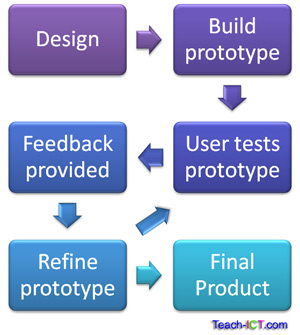
\includegraphics{figs/evolutionary.png}} 
    \caption{Modelo evolutivo\cite{Modeloevolutivo}} 
    \label{fig:Espiral} 
  \end{center} 
\end{figure}
Si se quiere entender un poco más este concepto de ciclo de vida en espiral, primero hay que comprender de qué trata. Si se compara con el desarrollo de un modelo en cascada, se puede ver que mientras en el modelo en cascada primero se buscan los requisitos, después se diseña la aplicación, se implementa y ya para finalizar se realizan las pruebas y el mantenimiento. 
En espiral primero se determinan objetivos que se quiere alcanzar en esa fase, tanto requisitos como restricciones. Después se desarrolla la aplicación y se realizan las pruebas. Una vez realizadas esas pruebas, se planifica lo que se va a realizar para la siguiente fase y lo que se dejará fuera del proyecto. 

\begin{figure}[H] 
  \begin{center} 
    \scalebox{1}{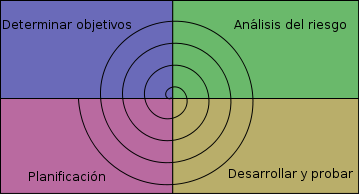
\includegraphics{figs/Espiral.png}} 
    \caption{Desarrollo en Espiral Wikipedia} 
    \label{fig:Espiral} 
  \end{center} 
\end{figure}

Durante cada una de las fases se determinaba un alcance y unas pruebas concretas.
Cada fase tiene un nombre propio con un significado especial, la primera fase se llama Tutorial, tiene este nombre ya que en esta fase se tuvo el contacto con las tecnologías y se empezó a trabajar con las APIs de Google. La segunda fase tiene como nombre Power-ups, este término tiene un significado propio en los videojuegos,  y se usa para identificar a los potenciadores que añaden capacidades adicionales a un personaje de un  videojuego, en este caso los power-ups fueron el feedback devuelto por los Baldusers. Para finalizar el nombre de la tercera fase es  Final Boss, ya que los nombres de las fases anteriores estaban identificadas por aspectos de videojuegos a esta última fase se le denomina así, puesto que el boss final de un videojuego es el jefe que hay que superar si se quiere dar como concluida la aventura que se empieza en el tutorial. En la tercera fase se dieron las últimas funcionalidades a Baldugenda y se preparó para la fase final de la aplicación.
\newpage
Ahora procederemos a explicar cada una de las fases seguidas durante el proyecto. Durante la explicación, se hará referencia a las fases del proyecto mediante los nombre propios explicados anteriormente. Siendo la primera fase Tutorial, la segunda Power-ups, y la tercera Final Boss.  
\begin{table} [H]
\centering
\resizebox{\textwidth}{!}{%
\begin{tabular}{@{}ccccc@{}}
\toprule
Fases  & \multicolumn{1}{l}{Nº personas} & Objetivos                                                                                                                              & Riesgos                                                                               & Desarrollo                                                                                           \\ \midrule
Tutorial & 2                               & \begin{tabular}[c]{@{}c@{}}Casos de uso básicos \\ (Exámenes, Asignaturas)\\ \acrshort{api} Google Calendar\\ Corrección  de errores\end{tabular} & API Google Calendar                                                                   & Objetivos implementados                                                                              \\ \midrule
Power-ups & 6                               & \begin{tabular}[c]{@{}c@{}}Modificaciones y Borrados\\ (Exámenes, Asignaturas)\\ Notas\\ Corrección de errores\end{tabular}            & \begin{tabular}[c]{@{}c@{}}Dos tipos de BD distintas\\ en funcionamiento\end{tabular} & \begin{tabular}[c]{@{}c@{}}Conversión de la BD\\ implementada\\ Objetivos implementados\end{tabular} \\ \midrule
Final Boss & 15                              & \begin{tabular}[c]{@{}c@{}}Backup\\ Descripción examen\\ Modificaciones App\\ Corrección de errores\end{tabular}                       & API Google Drive                                                                      & Objetivos implementados                                                                              \\ \bottomrule
\end{tabular}
}
\caption{Resumen fases de desarrollo}
\end{table}
 
\subsection{Tutorial}
\label{subsecc:Tutorial}

Para esta fase los Baldusers que estaban dentro del proyecto eran el tutor y el desarrollador de la aplicación. Las funcionalidades que se decidieron para esta primera fase fueron los casos básicos referentes a la creación de asignaturas y exámenes, dentro de estos casos básicos podemos encontrar la creación de una asignatura con una lista de enlaces y la selección del tipo de evaluación que tiene dicha asignatura. En cuanto a los exámenes, la creación de exámenes asociados a una asignatura con una fecha en concreto, y la hora en la que se realizaría.
También se decidió incluir el API de Google Calendar al proyecto, y con el API se incluyeron más funcionalidades como la creación de un evento dentro de un calendario de Google Calendar propiedad del usuario como recordatorio del examen. El usuario podría escoger si quiere notificaciones en ese evento o no, se agregó la  posibilidad de modificar los calendarios de Google propios del usuario dentro de la aplicación, y poder añadir o borrar calendarios existentes.
 
Dentro de la fase, aparte del alcance, hubo una parte de pruebas donde el tutor y yo usaríamos Baldugenda y comprobaríamos que funcionaba correctamente para proceder a pasar a la fase de Power-ups.
\newpage

\subsection{Power-ups}
\label{subsecc:Powerups}

Después de realizar la fase Tutorial, se revisaron las funcionalidades propuestas e implementadas durante la primera fase. A la hora de realizar esta revisión se separaron las propuestas en 3 bloques: a) uno para las funcionalidades que se mantendrían o se implementarían durante esta segunda fase, b) en el segundo bloque estarían las funcionalidades que o por falta de tiempo o complejidad se dejarían para fases siguientes, y c) en el bloque tres estarían las funcionalidades que quedarían fuera del proyecto porque se alejaban mucho de la idea inicial o por el coste que supondría hacerlas.
Las funcionalidades que se decidieron mantener de la primera fase fueron la mayoría, ya que al ser la primera fase,dichas funcionalidades eran  muy básicas como para poder desecharlas. Las implementaciones que se realizaron pero que no convencieron a los Baldusers de esa fase, se quitaron para el siguiente, y se decidió que si en el futuro hubiera tiempo, se volverían a incluir. Una de las funcionalidades que sufrió este cambio fue la de las notificaciones en los exámenes mediante Google Calendar. Durante el Tutorial se implementó para ver su funcionamiento, pero no convenció a los Baldusers y se retiró para el comienzo de Power-ups.

Para el alcance de esta fase, los Baldusers agregados probaron Baldugenda, y devolvieron el feedback sobre la aplicación que había resultado de Tutorial. Dentro de este feedback se les pidió que dijeran funcionalidades nuevas que podrían añadirse en Baldugenda. Surgieron bastantes funcionalidades, como pasó en Tutorial se volvió a dividir dichas funcionalidades en 3 bloques, y cuando se tuvo determinar los objetivos se escogió qué tipo de funcionalidades se realizarían en esta fase.
Para disponer de la información que devolvían los Baldusers de una manera rápida se decidió usar documentos de Google Drive y compartirlos a los Baldusers, ellos mismos irían rellenando lo que querían agregar a la aplicación, y después en la fase de toma de decisiones se escogería qué se dejaba fuera.

En el bloque de los casos de uso que se realizarían durante esta fase, se agregó que los usuarios pudieran modificar una asignatura o un examen. Por otro lado, también se decidió implementar que el usuario pudiese borrar las asignaturas que no tuvieran exámenes asociados. Como aspectos nuevos que se incluirían en Power-ups fueron: añadir nota en examen y en asignatura, y también solucionar los errores encontrados por los Baldusers cuando estaban realizando las pruebas.

En el apartado de diseño los Baldusers se quejaron y ellos mismos propusieron un diseño que les parecía más atractivo.
Hubo casos de uso y aspectos que se tuvieron que dejar fuera, como fue el caso de agregar nuevos eventos: las tutorías o trabajos grupales e individuales.
Las funcionalidades que los Baldusers sugirieron y que nos parecieron interesantes pero se realizarían más adelante fueron: la de agregar descripción en exámenes y realizar unos ajustes en la aplicación para que cuando se crease un examen o una asignatura, ésta se mostraría directamente sin tener que realizar una búsqueda después.

Durante la fase de análisis de riesgos se tuvo en cuenta que al ser una segunda versión de la aplicación, ya habría Baldusers que se la habían instalado, y que en sus dispositivos estaba una versión de base de datos con un esquema distinto del que se lanzaría en la nueva versión, por este motivo, lo primero que se llevaría a cabo sería el apartado de realizar una correcta transformación de la base de datos antigua a la nueva sin que los Baldusers perdieran la información almacenada hasta ese momento.

Para la parte de implementación se buscó la manera de que el Balduser que probara la aplicación no se viera afectado con los cambios realizados. Para conseguir ese objetivo el único aspecto de diseño que se modificó fueron los iconos del menú principal. También a la hora de implementar los nuevos campos de nota en examen y en asignatura, se tenía que tener en cuenta tanto a los Baldusers que habían probado la aplicación, como a los que la probarían en un futuro, por eso se tenía que tener en cuenta las dos situaciones que se podían dar cuando los Baldusers probaran la nueva versión. Podía darse el caso que el Balduser fuera nuevo o por el contrario ya la tuviera instalada y sólo tuviera que actualizarla.

Para la fase de pruebas se les informó a los Baldusers que ya podían actualizar Baldugenda a la nueva versión con los cambios que habían solicitado. En ese momento los Baldusers tenían que realizar pruebas, comprobar el diseño, e informar de  cualquier fallo que se produjese en la aplicación. La fase de pruebas era una fase importante en esta fase, ya que al haber agregado funcionalidades nuevas, tenían que funcionar correctamente si se quería empezar una fase nueva sin problemas. Durante la fase de pruebas no se encontraron fallos importantes, los fallos que se encontraron se pudieron solucionar antes de comenzar la nueva fase.
\newpage
\subsection{Final Boss}
\label{subsecc:final boss}

En esta fase el funcionamiento varió con respecto a los anteriores, hay que recordar que durante el Tutorial uno la cantidad de usuarios que podían usar la aplicación era un grupo reducido de una o dos personas, en Power-ups el grupo de usuarios pasó de ser de dos personas a ser 6, y en Final Boss se volvió a aumentar el grupo de Baldusers y se probó con 15 personas.

Para empezar, en esta fase se les permitió a los Baldusers descargar la aplicación que se había desarrollado hasta el momento en Power-ups, y se les pidió el feedback después de que realizaran unas pruebas, se cambió el método de adquirir la información de los Baldusers, ya que nos dimos cuenta que durante Power-ups el feedback producido por esos medios no fue suficientemente productivo. Por este motivo se les dio la posibilidad de ponerse en contacto conmigo tanto por teléfono, e-mail o en persona, para que me fueran informando de los cambios que veían necesarios para Baldugenda.
En algunos casos, cuando el Balduser pudo quedar conmigo se realizaron una serie de pruebas para saber cómo interactuaba el Balduser con la aplicación, una de esas pruebas era la de tener que realizar una serie de acciones con Baldugenda, y se le iban contando las pulsaciones que realizaba y el tiempo que le llevaba realizar cada tarea.

Los Baldusers respondieron mejor que la vez pasada, aunque hubo más problemas a la hora de instalar la aplicación ya que el tipo de usuario que se escogió fue un tipo de usuario que no tenía conocimientos de informática, esto repercutió en el tiempo que necesitaban para instalarse la aplicación. Del feedback que se recibió de los Baldusers, se incluyó en la implementación de esta fase el apartado de poder realizar un backup de la información, para después poder recuperarla. También se agregó la descripción dentro de examen, esta funcionalidad estaba presente en el feedback de los usuarios de Power-ups pero por tiempo no se pudo incluir. La mayoría de las funcionalidades que se modificaron fueron cambios en el funcionamiento en la interacción con la aplicación, cambios del tipo pulsación de los botones o nuevos accesos a los casos de uso ya implementados. Se dejaron casos de uso fuera, como fue el caso de modificar todo el diseño de la aplicación que se dejó para las siguientes fases.

En la fase de análisis de riesgos se tomó en cuenta que al querer implementar el backup con un servicio de Google, el API de Google Drive,  las dificultades que podían salir a la hora de trabajar con una tecnología que no se conocía de antes, se solventarían atrasando el caso de uso del backup a una fase posterior, siempre y cuando esas dificultades produjesen un coste superior al planificado durante la fase, si no se consiguiera implementar con la tecnología de Google, se realizarían backups de manera alternativa.

En la fase de implementación se desarrolló con éxito el apartado del backup con unos pequeños problemas al principio, los cuales por medio de documentación oficial se consiguió arreglar. Dentro de la fase de implementación tuvimos en cuenta que en ese momento podían existir 3 versiones de la aplicación: la versión de Tutorial, la de Power-ups y la versión actual de Final Boss, así que había que tener cuidado con esa cuestión, ya que la aplicación tenía que seguir funcionando daba igual desde qué versión se llegara. Cuando se acabó la implementación se subió a Google Play para compartir con los Baldusers la nueva versión, se la descargaron y realizaron unas pruebas para encontrar fallos. Todos los fallos que se fueron encontrando hasta la fecha se fueron resolviendo en una versión nueva cada semana.

Los objetivos que se marcaron para dar conclusión a Final Boss fueron: el de alcanzar una versión estable del producto, e implementar las funcionalidades que se habían decidido incluir durante las tres fases. A partir de la tercera fase, Baldugenda está recibiendo actualizaciones. Cuando los Baldusers encuentran fallos se realiza un mantenimiento de la aplicación y se vuelve a subir la nueva versión a Google Play . 
\newpage
\section{Participación de los usuarios en el proyecto}
\label{secc:Participación de los usuarios en el proyecto}

Ya se ha ido comentando cómo dentro de cada fase se iba cambiando el número de Baldusers, las labores que realizaron los Baldusers fueron de distintos ámbitos. Hubo Baldusers que no devolvieron un feedback importante en cuanto a nuevas funcionalidades pero sí que fueron reportando cada fallo que se producía en la aplicación. 
Aparte de los feedbacks que iban realizando, también se realizaron unas pruebas con alguno de ellos, de estas pruebas se pudieron sacar datos interesantes en cuanto al uso de los usuarios dentro de un proyecto software destinado a móviles, como puede ser la edad o los conocimientos informáticos.

Para recopilar toda la información que aportaban los Baldusers se usaron cuestionarios, durante la primera fase se les pedía que los rellenaran, en cambio a partir de la segunda fase los cuestionarios los iba rellenando yo a medida que me iban diciendo el feedback por lo medios que vieran mas oportunos. Estos cuestionarios constaban de una serie de preguntas sobre lo que les parecía Baldugenda y que aspectos tanto de diseño, como funcionales les gustaría que cambiasen para futuras versiones.Dentro de las pruebas se les daba una serie de puntos que debían realizar mediante Baldugenda, para ver como se desenvolvían con la aplicación. Una vez se realizaban los cambios que pedían los usuarios se les informaba de una nueva versión y volvían a informar sobre posibles mejoras y cambios. 

La información  que aportaban variaba mucho dependiendo del tipo de usuario que la escribiera. Dentro del capítulo de usuarios se desarrollará los tipos de usuarios encontrados durante las fases del proyecto y las ventajas de colaborar con unos u otros.

En el capítulo de usuarios se detallará en profundidad el tipo de documentos que se usó para realizar las encuestas y para recoger el feedback. También en este capítulo se podrá encontrar los medios de comunicación usados con los usuarios y problemas encontrados.
\nocite{*}


% Mediante los siguientes comandos, podrás compilar el conjunto de ficheros desde este mismo documento


%%% Local Variables: 
%%% mode: latex
%%% TeX-master: "../Principal"
%%% End: 


















% line in order to check if utf-8 is properly configured: áéíóúñ